\chapter{Background} 
\label{chapter:background}

In information reterval one of the most easiest approaches of finding relevant documents given a query is TFIDF.
TFIDF,short for term frequency-inverse document frequency, is a information retrieval technique that shows how important a word is to a document. Another information retieval function known as BM25 (BM stands for Best Match) \cite{robertson2009probabilistic}can be used to retreive matching documents according to their relevance to a given query.\cite{dumais2004latent} introduced a word embedding method as an extension of TDIDF known as Latent Semantic Analysis(LSA). LSA is essentailly a statistical method, other word embedding models such as  Word2Vec \cite{mikolov2013efficient}  ,Glove \cite{pennington2014glove} and Swivel \cite{shazeer2016swivel} have now become a benchmark in semantic similarity extraction.


\section{Summary of relevant approaches}
TFIDF is an information retrieval technique that calculates a a given terms frequency(TF) and its inverse document frequency(IDF). Each word or term has its own TF and IDF score, the product of the two scores is called the TFIDF weight of that term.\cite{ramos2003using} provide evidence that TFIDF returns
documents highly correlate to the given query.Different weight schemes for these counts lead to a variety of TF-IDF ranking features. One very successful TF-IDF
formulation is known as BM25\cite{robertson2009probabilistic}.
BM25  is a bag-of-words information retrieval function that ranks a set of documents based on their relevance to the query terms. Tweaking different components and parameters produce different variations of the BM25. \cite{mitra2016dual} have shown BM25 to be effective in information retrieval and have also proposed using it in an ensemble model along with other embedding model, namely Word2Vec.

The TF-IDF vectors tend be large since they have one component for every word in the vocabulary. \cite{berger2000bridging} propse a number of extentions to TFIDF, including what they call Adaptive TFIDF. This algorithm incorporates hillclimbing and gradient descent to improve the performance.

Another extension introduced by \cite{dumais2004latent} is known as LSA.
LSA uses Singular Value Decomposition(SVD) to perform dimensionality reduction on the TF-IDF vectors resulting in smaller and better features.
\cite{boling2014semantic} has shown that LSA performs very well in finding semantic similarity between documents and its terms
As of late, the most used and
powerful representations are one of the following embeddings: Word2Vec \cite{mikolov2013efficient} 
and GloVe \cite{pennington2014glove}, which are word level embeddings
\subsection{Word Embeddings} 
Word embedding is a language modeling and feature learning technique in natural language processing(NLP) which maps words and phrases to the real number vector space of desired dimension. 

\paragraph{Word2Vec} Word2Vec model uses distributed vector representation of words, a well-known framework for learning word vectors as shown in the Figure \ref{fig:Word2Vec model}. The task is to learn to predict a word given other words in the context.
More formally, given a sequence of training words
$w_{1}, w_{2}, w_{3}, ..., w_{T} $, the objective of the word vector model is to maximize the average log probability
\\
\begin{equation}
\frac{1}{T} \sum_{t=K}^{T-K} \log p(w_{t} \mid w_{t-1},....,w_{t+1}) 
\end{equation}

\begin{figure}[h]
	\centering
	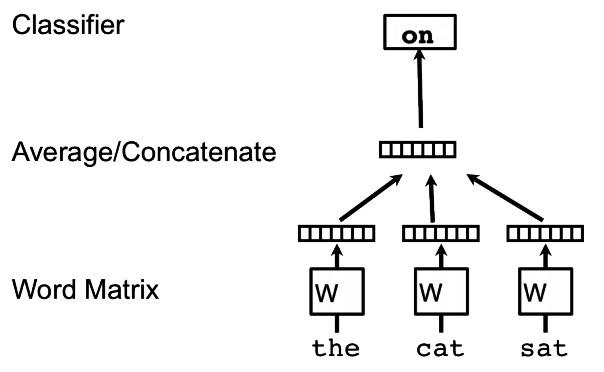
\includegraphics[width=8cm, height=5cm]{w2v.png}
	\caption{A framework for learning word vectors. Context of
		three words (“the,” “cat,” and “sat”) is used to predict the fourth
		word (“on”). The input words are mapped to columns of the matrix
		W to predict the output word.}
	\label{fig:Word2Vec model}
\end{figure}


 \cite{bojanowski2016enriching} propose another extention of Word2Vec model known as FastText. It learns word
 representations while taking into account morphology.
 FastText models morphology by considering subword
 units, and representing words by a sum of its character
 n-grams.  Since FastText exploits subword information, It can also
 compute valid representations for out-of-vocabulary
 words. FastText obtains representations for out-of-vocabulary words by summing the vectors of character
 n-grams
 
 \cite{joulin2016fasttext} propose a memory efficient extension of FastText. They propose using product quantization to store word embeddings.
 
 \cite{ghosh2016characterizing} introduce a vocabulary driven Word2Vec method known as Dis2Vec which is
 used to generate disease-specific word embeddings from unstructured health-
 related news corpus. The input corpus D consists of a collection of word context pairs.The input corpus $D$ consists of a collection of word context pairs. Based on the vocabulary $ V$, we can categorize the word context pairs into three types as shown
 below:
 \\
 \begin{itemize}
 	\item $ D(d) = {(w, c): w \in V ∧c \in V }$, i.e. both the word w and the context c are in V
 	\item $D(\rightharpoondown d) = {(w, c): w \notin V ∧c \notin V }$, i.e. neither the word w nor the context c are in V
 	\item $D(\rightharpoondown d) = {(w, c): w \in V \oplus c \in V }$, i.e. either the word w is in V or the context c is in V but both cannot be in V
 \end{itemize}
 
 Each of these categories of (w, c) pairs
 needs special consideration while generating disease specific embeddings.
 
 
 All the above mentioned word embedding models learn word embeddings from co-occurrence information in corpora.
 One drawback of learning word embeddings by by this approach is that such methods will generally fail to tell synonyms from
 antonyms (Mohammad et al., 2008). For example, words like east and west
 or expensive and cheaper appear in near-identical contexts, which means
 that distributional models produce very similar word vectors for such words.
 \cite{mrksic:2016:naacl} proposed a novel counter-fitting method which injects antonymy and
 synonymy constraints into vector space representations in order to circumvent this issue.\ref{tab:counter_fitting} shows the results \cite{mrksic:2016:naacl} achieved using their counter-fitting technique.
 
 \begin{table}[h]
 	\begin{center}
 		\begin{tabular}{ c c c c } 
 			\hline
 			& east & expensive & British \\
 			\hline
 			\multirow{5}{4em}{Before} &
 			
 			west & pricey &  American
 			\\ 
 			& north & cheaper & Australian\\ 
 			& south & costly & Britain\\ 
 			& southeast & overpriced & European\\
 			& northeast & inexpensive & England\\
 			\hline
 			\multirow{5}{4em}{After} & 
 			eastward & costly & Brits\\ 
 			& eastern & pricy & London\\ 
 			& easterly & overpriced & BBC\\ 
 			& - & pricey & UK\\ 
 			& - & afford & Britain\\ 
 			\hline
 		\end{tabular}
 		
 	\end{center}
 	
 	\caption{Nearest neighbours for target words using GloVe
 		vectors before and after counter-fitting} \label{tab:counter_fitting}
 \end{table}
 
 An alternative to
 the bag-of-words approach is to derive contexts
 based on the syntactic relations the word participates
 in as proposed by \cite{levy2014dependency}.


\paragraph{Doc2Vec}Doc2Vec is capable of constructing representations of input sequences of
variable length. Unlike some of the previous approaches, it is general and
applicable to texts of any length: sentences, paragraphs, and documents. In
Doc2Vec framework (see Figure \ref{fig:doc2vec model}), every document is mapped to a unique
vector, and every word is also mapped to a unique vector. The document
vector and word vectors are averaged or concatenated to predict the next
word in a context. The only difference to a Word2Vec model is the additional
document token.It acts as a memory that remembers what is missing from
the current context or the topic of the document. The document vectors and
word vectors are trained using stochastic gradient descent and the gradient
is obtained via back-propagation.

\begin{figure}[h]
	\centering
	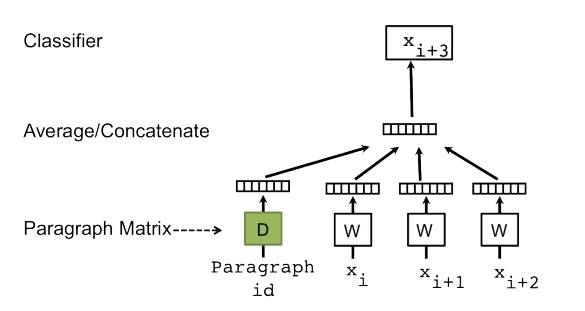
\includegraphics[width=8cm, height=5cm]{para}
	\caption[]{A framework for learning paragraph vector. This framework
		is similar to the framework presented in Figure 1; the only
		change is the additional paragraph token that is mapped to a vector
		via matrix D. In this model, the concatenation or average of
		this vector with a context of three words is used to predict the
		fourth word. The paragraph vector represents the missing information
		from the current context and can act as a memory of the
		topic of the paragraph.}
	\label{fig:doc2vec model}
\end{figure}

An extension to Word2Vec
known as Doc2Vec was proposed in /////. 



	